\section{李群与李代数}


\subsection{快速问答}
\begin{itemize}
    \item 李群和李代数主要解决的问题是什么?{\color{blue} 李群和李代数将一个乘法运算群转换成加法运算,通过加法运算,我们能更方便的使用微分和梯度进行寻找极值点。}
    \item 为什么我们需要使用微分?{\color{blue} 在优化问题中,往往我们不能直接找到函数的极值点,一般来说,我们通过梯度下降的方式找到函数的极值点。梯度下降要求我们对变量求导,得到梯度\(\Delta x\),在每次迭代中使用\(x+\Delta x\)作为下一步的函数值进行优化。}
    \item 为什么在SLAM优化问题中使用李群?{\color{blue} SLAM的位姿求解包含了俩个重要的矩阵,旋转矩阵\(R\)和变换矩阵\(T\)。然而这俩个矩阵对加法不封闭,他们都是乘法群。为了能获得梯度下降,我们需要将乘法群转换成加法群。}
    \item 乘法如何转换成加法?{\color{blue} 在标量运算中,我们有一个很漂亮的形式,\(f(x)=e^x\),我们有\(f(a)f(b)=f(a+b)\)。通过指数或者对数映射,我们能够将一个乘法运算转换成加法运算。因此,我们的目标是利用李群和李代数寻找矩阵的某种指数和对数映射关系。}
    \item 什么是矩阵指数?{\color{blue} 我们定义矩阵指数\(e^A\),对于标量来说,我们有\(e^0=1\),\(e^{a+b}=e^ae^b\)。在矩阵指数中,我们也应该满足类似的性质。}
\end{itemize}


\subsection{旋转矩阵的求导}
考虑任何一个旋转矩阵\(R\),我们知道旋转矩阵满足
\[
    RR^T = I
\]
考虑一个连续变换的旋转矩阵\(R(t)\),其中\(t\)表示时间参数,根据上述的方程我们可知
\[
    R(t)R(t)^T = I
\]
我们对方程两侧求导可知
\[
    R'(t)R(t)^T + R(t)R'(t)^T=0
\]
整理得到
\[
    R'(t)R(t)^T = -R(t)R'(t)^T = -(R'(t)R(t)^T)^T
\]
因此我们得到矩阵\(R'(t)R(t)^T\)是一个反对称矩阵。对于任意一个反对称矩阵来说,其对角元素为\(0\),且对角线元素为相反数。我们可以找到一个唯一对应的向量,并用运算符\(\wedge\)和\(\vee\)表示向量和矩阵的转换关系
\[
    a^\wedge = A = \begin{bmatrix}0 & -a_3 & a_2\\a_3 & 0 & -a_1\\-a_2 & a_1 & 0\end{bmatrix}, A^\vee = a
\]
所以我们可以找到一个三维向量\(\phi(t)\),使得{\color{red} \(R'(t)R(t)^T=\phi(t)^\wedge\)}。两边同时乘以\(R(t)\),我们得到
\[
    R'(t)R(t)^TR(t) = {\color{red} R'(t) = \phi(t)^\wedge R(t)}
\]
由此我们得到了在\(t\)时刻,旋转矩阵的导数与旋转矩阵的关系。
现在我们考虑{\color{blue} 泰勒定理},对于函数\(f(x)\)在\(a\)附近的值,我们有
\[
    f(x) \approx f(a) + f'(a)(x-a)
\]
我们将函数\(R(t)\),和\(a=0\)代入泰勒定理,且我们让旋转矩阵初值为单位矩阵\(I\),我们得到\(R(t)\)在\(t=0\)附近的值为
\[
    R(t) \approx R(0) + R'(0)t = I + \phi(0)^\wedge I t = I + \phi(0)^\wedge t
\]
由此可见在原点附近,函数\(R(t)\)的导数在正切空间上。
{\color{red} 暂时未能有明确解释:由此我们可见\(\phi(t)^\wedge\)在\(t=0\)附近几乎保持不变,我们可以假设其在\(t=0\)附近时,保持为常数\(\phi_0\)。由此我们得到在\(t=0\)附近时,我们有}
\[
    R'(t) \approx \phi_0 R(t)
\]
这是一个很简单的微分方程,一个函数的导数等于其函数本身,我们很容易联想到指数函数,因此,我们可以得到其原函数为
\[
    R(t) \approx e^{\phi_0 t}
\]


\subsection{李代数的引出}
所有的旋转矩阵构成了群
\[
    SO(3) = \{R \in \mathbb{R}^{3x3} | RR^T = I, det(R) = 1\}
\]
所有的变换矩阵构成了群
\[
    SE(3) = \{T = \begin{bmatrix} R & t \\ 0^T & 1\end{bmatrix} \in \mathbb{R}^{4x4} | R \in SO(3), t \in R^3\}
\]
在\(SO(3)\)群和\(SE(3)\)群上,其都对乘法封闭,但对加法不封闭。
\begin{definition}
    李群是指具有连续光滑性质的群。
\end{definition}
很显然\(SO(3)\)群和\(SE(3)\)群在实数空间上连续且平滑,因此他们都是李群。\\
现在我们引入李代数,,每个李群都有与之对应的李代数。李代数描述了李群的局部性质,准确的说,是单位元附近的正切空间(正是函数\(R(t)\)的样子),一般李代数的定义如下:
\begin{definition}
    对于一个集合\(\mathbb{V}\),数域\(\mathbb{F}\),以及一个二元运算\([,]\),有
    \begin{itemize}
        \item 封闭性,\(\forall X, Y \in \mathbb{V}, [X, Y] \in \mathbb{V}\)
        \item 双线性,\(\forall X, Y, Z \in \mathbb{V}, a, b \in \mathbb{F}\),有
              \[
                  [aX + bY, Z] = a[X, Z] + b[Y, Z]; [Z, aX + bY] = a[Z, X] + b[Z, Y]
              \]
        \item 自反性,\(\forall X \in \mathbb{V}, [X, X]=0\)
        \item 雅可比等价,\(\forall X, Y, Z \in \mathbb{V}, [X, [Y, Z]] + [Z, [X, Y]] + [Y, [Z, X]] = 0\)
    \end{itemize}
\end{definition}
二元运算又被称为李括号,粗看起来,李代数需要的性质还是挺多的,实际上,三维向量\(\mathbb{R}^3\)定义的的叉积是一种李括号,因此\((\mathbb{R}^3, \mathbb{R}, x)\)构成了一个李代数。{\color{red} 实际上,向量\(\phi\)也是一个李代数。}
\begin{definition}
    我们定义\(\Phi = \phi^\wedge\),以及李括号
    \[
        [\phi_1, \phi_2] = (\Phi_1\Phi_2-\Phi_2\Phi_1)^\vee
    \]
\end{definition}
不难验证,\(\phi\)是一个李代数,其和李群\(SO(3)\)的对应关系为
\[
    R = e^{\phi^\wedge}
\]


\subsection{矩阵的指数对数映射}
刚刚我们得到了在局部范围的旋转矩阵的指数形式,
\begin{definition}
    矩阵的指数定义,设矩阵\(A\)为方阵,则
    \[
        e^A = \sum_{n=0}^{\infty}\frac{1}{n!}A^n
    \]
\end{definition}
然而,我们并不想引入无穷项的计算,对于李代数\(\phi\)来说,由于它是一个向量,我们可以定义\(\phi=\theta \mathbf{a}\),其中\(\mathbf{a}\)为单位向量,\(\theta\)为模。我们发现
\[
    \mathbf{a}^\wedge \mathbf{a}^\wedge = \mathbf{a} \mathbf{a}^T - I \\
    \mathbf{a}^\wedge \mathbf{a}^\wedge \mathbf{a}^\wedge = - \mathbf{a}^\wedge
\]
代入指数映射\(R = e^{\phi^\wedge}\),我们得到
\[
    e^{\phi^\wedge}=cos \theta I + (1-cos \theta)\mathbf{a} \mathbf{a}^T + sin \theta \mathbf{a}^\wedge
\]
总结李代数和原旋转矩阵的映射关系,我们有
\begin{figure}[H]
    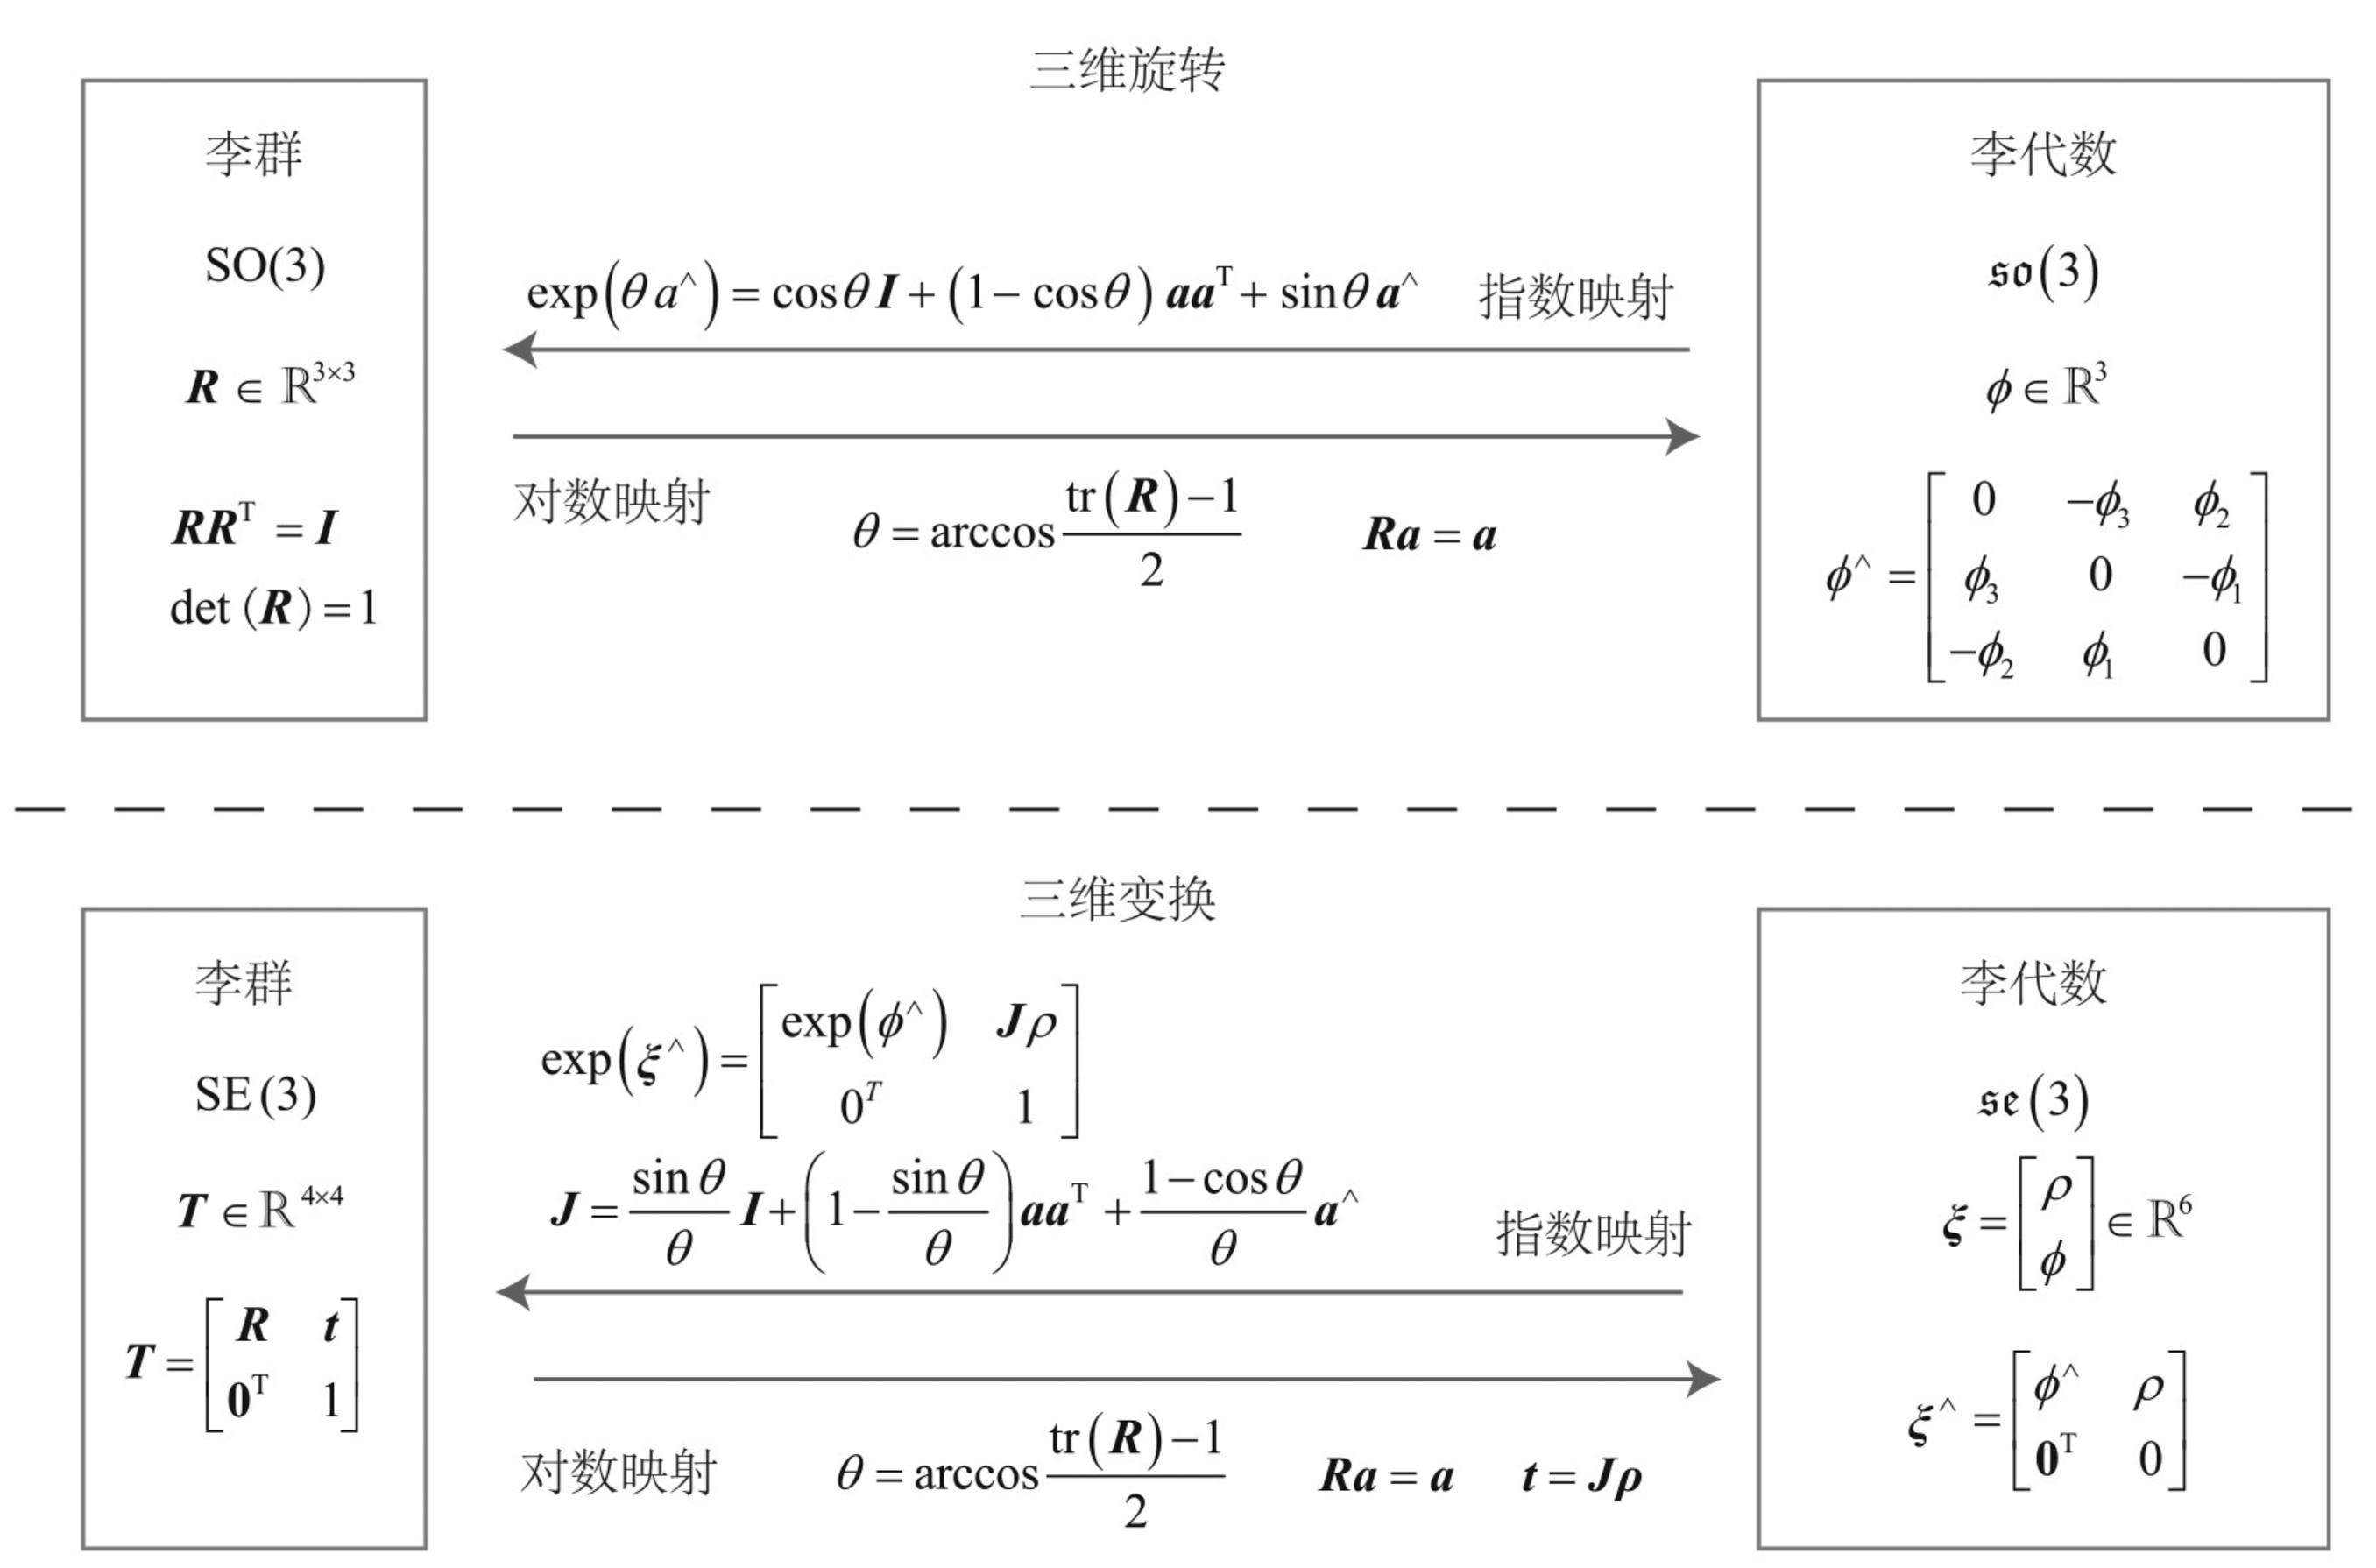
\includegraphics[width=1\linewidth]{images/lie-rotation-transformation.png}
    \label{fig:enter-label}
\end{figure}


\subsection{李代数求导与扰动模型}
引入李代数是为了求导,然而李代数指数映射乘积的完整形式并不像普通的标量指数那么简单,这里有一个微小的扰动,其方程可以写成
\[
    ln(e^{\phi_1^\wedge}e^{\phi_2^\wedge})^\vee \approx \left\{ \begin{array}{cc} J_l(\phi_2)^{-1}\phi_1 + \phi_2 \text{\quad\quad 当\(\phi_1\)为小量}\\ J_r(\phi_1)^{-1}\phi_2 + \phi_1 \text{\quad\quad 当\(\phi_2\)为小量} \end{array} \right.
\]
其中
\[
    J_l=\frac{sin \theta}{\theta}I + (1-\frac{sin \theta}{\theta})\mathbf{a}\mathbf{a}^\wedge + \frac{1-cos \theta}{\theta}\mathbf{a}^\wedge
\]
\[
    J_r(\phi)=J_l(-\phi)
\]
终于,我们可以将旋转矩阵的乘法转换成李代数的加法。{\color{red} 对于一个旋转矩阵\(R\)来说,当我们左乘一个小的变化量\(\Delta R\),我们有}
{\color{red}
\[
    \Delta R R = e^{\Delta \phi^\wedge}e^{\phi^\wedge} = e^{(\phi + J_l(\phi)^{-1}\Delta\phi)^\wedge}
\]}



\subsection{SLAM中的位姿优化问题和李代数求导}
我们首先来考虑下SLAM中的位姿优化问题。假设某个时刻,相机的位姿态为\(T\),对于世界坐标中的一个点\(p\)来说,产生了一个观测数据\(z\),很显然\(z=Tp\)。然而由于噪声的存在,通常\(e = z-Tp \neq 0\)。对于位姿优化问题来说,对于N个这样的路标点和观测,我们寻找
\[
    \mathop{argmin}\limits_{T} \sum_{i=1}^N ||z_i - Tp_i||^2_2
\]
我们用左乘\(\Delta R\)作为扰动,并且设\(\Delta R\)的李代数为\(\varphi\),换言之\(\Delta R = e^{\varphi^\wedge}\),那我们有
\[
    \frac{\partial Rp}{\partial \Delta R} = \frac{\partial Rp}{\partial \varphi} = \mathop{lim}\limits_{\varphi \rightarrow 0}\frac{e^{\varphi^\wedge} e^{\phi^\wedge} p - e^{\phi^\wedge} p}{\varphi} = -(Rp)^\wedge
\]
同样我们可以把求导扩展到\(SE(3)\)群上,我们有
\[
    \frac{\partial Tp}{\partial \Delta T^\vee} = \begin{bmatrix}I & -(Tp)^\wedge \\ 0^T & 0^T\end{bmatrix}
\]